\documentclass{article}
\usepackage[hidelinks]{hyperref}
%\usepackage{helvetica} % uses helvetica postscript font (download helvetica.sty)
%\usepackage{newcent}   % uses new century schoolbook postscript font 
%\setlength{\textwidth}{5.5in} % set width of text portion
\usepackage{graphicx}
\usepackage{polski}
\usepackage{bm}
\usepackage{amsfonts}
%\usepackage[polish, english]{babel}
%\usepackage[T1]{fontenc} % T1, OT4
\usepackage[utf8]{inputenc}
\usepackage{indentfirst}
\usepackage{float}
\usepackage{enumitem}

\title{Projekt aplikacji do ekstremalnego uczenia maszynowego do klasyfikacji big data}
\author{Abdelkarim Ahmed, Hernik Aleksandra}
\date{}
\begin{document}

\clearpage
\vspace*{\fill}
\begin{center}
\begin{minipage}{.9\textwidth}
\maketitle
\end{minipage}
\end{center}
\vfill % equivalent to \vspace{\fill}
\clearpage

\tableofcontents
\clearpage

\section*{Wprowadzenie}
\addcontentsline{toc}{section}{Wprowadzenie}
Celem pracy jest przetestowanie ELM na wybranych zestawach small data, a następnie big data, przy użyciu służących do tego, istniejących już bibliotek do Pythona i Matlaba.

Ahmed Abdelkarim zajmował się porównywaniem wyników dla big data i~small data przy użyciu Pythona.
Aleksandra Hernik sprawdzała dokładność i~wydajność uczenia dla big data za pomocą Matlaba.

\clearpage
\section*{Wykaz ważniejszych oznaczeń i akronimów}
\addcontentsline{toc}{section}{Wykaz ważniejszych oznaczeń i akronimów}
\begin{itemize}[label={},leftmargin=*]
\item ELM -- \textbf{E}xtreme \textbf{L}earning \textbf{M}achine - ekstremalne uczenie maszynowe
\item SLFN -- \textbf{S}ingle-\textbf{L}ayer \textbf{F}eed-forward \textbf{N}etwork - jednowarstwowa jednokierunkowa sieć neuronowa
\item BP -- \textbf{B}ack-\textbf{p}ropagation - propagacja wsteczna
\item MLP -- \textbf{M}ulti\textbf{l}ayer \textbf{P}erceptron - perceptron wielowarstwowy
\item SVM -- \textbf{S}upport \textbf{V}ector \textbf{M}achine - maszyna wektorów nośnych
\item Bias -- wyraz wolny, czyli dodatkowy neuron w warstwie wejściowej niewynikający z danych wejściowych, generujący zawsze +1, ale posiadający wagę
\item Big Data -- dane z liczbą próbek tak dużą, że nie występuje efekt przeuczenia
\item Small Data -- dane, dla których jest za mało próbek, aby sieć poznała dokładnie model bez przeuczenia
\item Toolbox -- zbiór funkcji stworzonych we wspólnym celu; biblioteka
\end{itemize}
\clearpage
\section{Opracowanie modelu pracy sieci do ekstremalnego uczenia maszynowego ELM}
\subsection{Rys historyczny}
Sieci neuronowe znajdują coraz to nowe zastosowania i stają się jednym z najważniejszych kierunków rozwoju informatyki. Jednak ograniczeniem tej metody jest długotrwały proces uczenia.

W 2004 roku w pracy \textit{Extreme Learning Machine: A New Learning Scheme of Feedforward Neural Networks} Guang-Bin Huang, Qin-Yu Zhu i Chee-Kheong Siew zaproponowali koncepcję ELM, mającą być rozwiązaniem tego problemu. Publikacja ta dotyczyła zastosowania ELM w SLFN. Przedstawiała podstawy teoretyczne do zastosowania tej metody, a także dowodziła zalet tego rozwiązania. Należą do nich wspomniana prędkość uczenia

W tym samym roku Guang-Bin Huang i Chee-Kheong Siew zaproponowali również w artykule \textit{Extreme Learning Machine: RBF Network Case} wariant ELM dotyczący sieci radialnych, których nie dotyczy ta praca. 

Kolejną istotnym wkładem tych autorów do tematu ELM jest opublikowany w 2005 artykuł \textit{Extreme Learning Machine: Theory and Applications}. Prezentowane są w nim wyniki ELM dla testowych danych, które pokazują, że metoda ta pozwala na dobrą klasyfikację, a może działać nawet kilka tysięcy razy szybciej niż tradycyjne metody. Od tego czasu pojawiło się wiele innych prac dotyczących tego zagadnienia, a zagadnienie stało się popularnym tematem.

Z wyżej wymienionymi pracami związane są kontrowersje dotyczące rzeczywistej innowacyjności rozwiązania Huanga i innych, a także oskarżenia dotyczące plagiatowania i nieuwzględniania w bibliografii rzeczywistych głównych źródeł pracy -- według nich artykuł dotyczący SLFN opiera się głównie na pracy \textit{Feed Forward Neural Networks With Random Weights} Woutera Schmidta, Martina Kraaijvelda i Roberta Duina z 1992, a artykuł dotyczący sieci radialnych wzoruje się na \textit{Multivariable Functional Interpolation and Adaptive Networks} Davida Broomheada i Davida Lowe'a. Huang wskazał pewne różnice między tymi pracami.
\subsection{Założenia dla sieci neuronowych klasy ELM}
Rozważane tu ELM zaliczają się do kategorii SLFN -- poza warstwą wejściową i wyjściową posiadają tylko jedną warstwę ukrytą. Od innych SLFN odróżnia je to, że ELM opierają się na losowym generowaniu neuronów warstwy ukrytej bez późniejszego ich dostosowywania do danych -- dzięki temu, że wszystkie ich parametry, takie jak np. wagi wejściowe, mogą zostać dobrane losowo, są one niezależne od danych trenujących, a w przeciwieństwie do metody BP, wagi wyjściowe są niezależne od wag wejściowych, co pozwala na nieiteracyjne ich wyznaczenie. Takie rozwiązanie zapewnia o kilka rzędów wielkości szybszy czas działania od innych metod, takich jak BP, MLP i SVM. 

\begin{figure}[H]
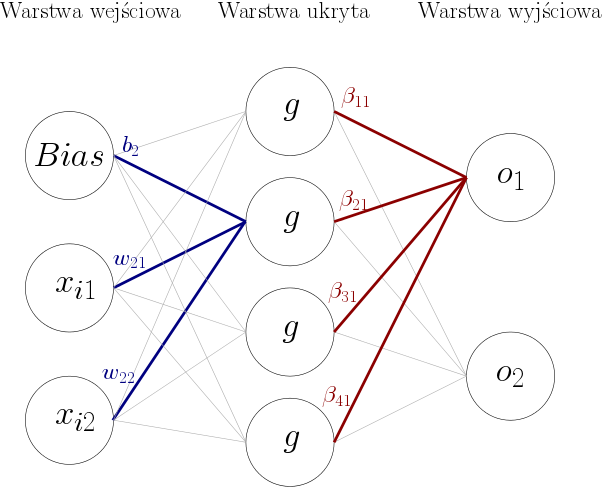
\includegraphics[width=\textwidth]{schemat_sieci.png}
\caption{Schemat SLFN typu ELM}
\end{figure}

Niech $N$ to liczba próbek danych trenujących postaci $(\bm{x}_i, \bm{t}_i) \in \mathbb{R}^n \times \mathbb{R}^m$, gdzie $\bm{x}_i = [x_{i1}, x_{i2}, \dots,  x_{in}]^T$ to dane wejściowe, a $\bm{t}_i = [t_{i1}, t_{i2}, \dots,  t_{im}]^T$ to oczekiwane wyniki. Wtedy dla SLFN z $\bar{N}$ ukrytymi neuronami wyjście dla i-tej próbki danych $(i=1,\dots,N)$ można zapisać jako:
$$\sum_{j=1}^{\bar{N}} \bm{\beta}_j g (\bm{w}_j \cdot \bm{x}_i + b_j)  = \bm{o}_i$$
gdzie $\bm{w}_j = [w_{j1}, w_{j2},\dots,w_{jn}]^T$ to wektor wag łączących warstwę wejściową z j-tym 

Możliwości uczenia się ELM zależą między innymi od doboru funkcji transformacji -- w szczególności ważne jest, żeby była ona nieliniowa, ponieważ to jedyne miejsce w całym modelu, w którym może być wykorzystane jakiekolwiek nieliniowe przekształcenie. Możliwe jest wykorzystanie różnych funkcji w różnych neuronach. Dla optymalnej jakości uczenia ważne jest również znormalizowanie danych wejściowych -- jeśli charakterystyki danych wejściowych mają różne rzędy wielkości, relatywnie drobne zmiany większej wartości mogą mieć większe znaczenie niż stosunkowo duże zmiany mniejszych wartości. Normalizacja pozwala na zrównanie wagi zmian wszystkich charakterystyk. \par

W przypadku problemu klasyfikacji, który jest rozważany w tej pracy, rozwiązaniem jest kategoria, dla której wartość na węźle wyjściowym była największa. 
\subsection{Wnioski i uwagi}
Ponieważ ELM jest bardzo szybką metodą, naturalne jest zastosowanie jej do big data -- przy czym tutaj big data oznacza dane takie, że liczba próbek jest wystarczająca, żeby wytrenować sieć bez przeuczania jej, a ograniczeniem jest tylko czas. W przypadku small data próbek jest za mało, żeby sieć mogła dokładnie nauczyć się modelu bez przeuczania. Szybkość uczenia w przypadku big data jest dodatkowo ograniczona sprzętowo -- danych jest zbyt dużo, żeby wszystkie zmieścić do pamięci operacyjnej komputera, co spowalnia dostęp do nich.

\clearpage
\section{Wykonanie implementacji ELM w Pythonie i Matlabie}
\subsection{Założenia dotyczące aplikacji}

Aplikacje udostępniają następujące funkcjonalności:
\begin{itemize}
\item Przygotowanie danych trenujących i testowych w formie plików csv
\item Trenowanie sieci neuronowej o architekturze ELM
\item Klasyfikacja danych testowych przez wytrenowaną sieć
\item Porównywanie wyników klasyfikacji do spodziewanych rezultatów
\item Analiza jakości klasyfikacji i  czasu trwania treningu
\item Interfejs graficzny
\end{itemize}
\begin{figure}[H]
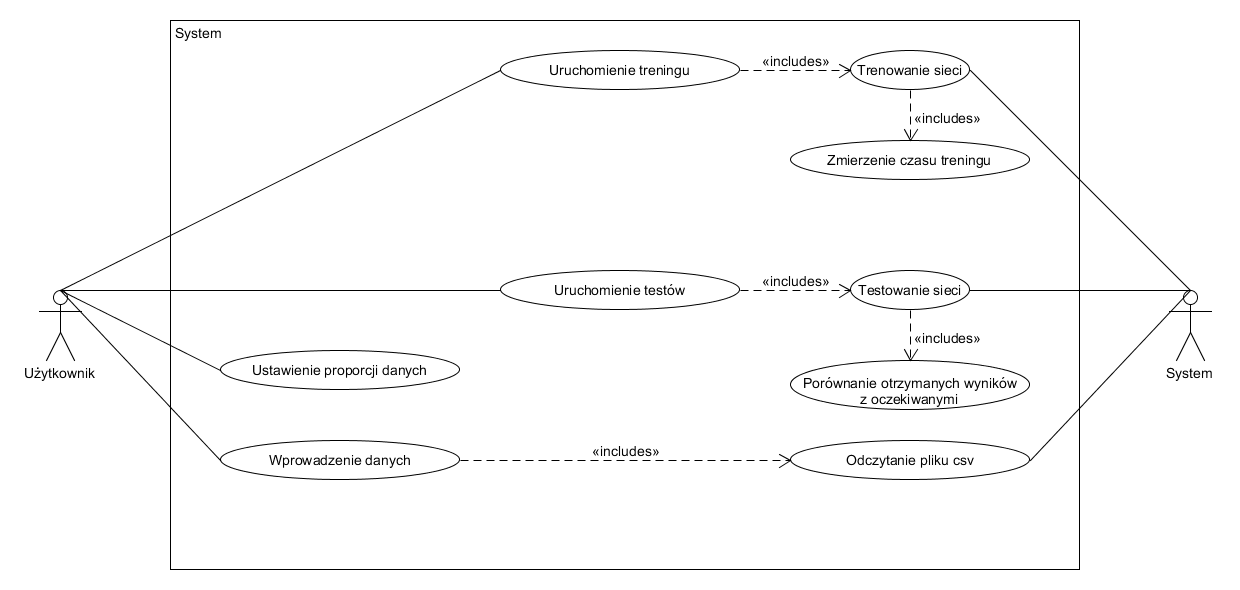
\includegraphics[width=\textwidth]{use_case.png}
\caption{Diagram przypadków użycia}
\end{figure}
\subsection{Projekt aplikacji sieci ELM w Pythonie}
\subsection{Projekt aplikacji sieci ELM w Matlabie}
\subsection{Wnioski i uwagi}
\clearpage
\section{Trening ELM dla wybranych benchmarków big data i small data}
\subsection{Opis wybranych benchmarków}
\subsection{Trening dla instancji klasy small data}
\subsection{Trening dla instancji klasy big data}
\subsection{Wnioski i uwagi}
\clearpage
\section{Eksperymenty obejmujące instancje klasyfikacji wraz z badaniem ich wydajności}
\clearpage
\section*{Podsumowanie}
\addcontentsline{toc}{section}{Podsumowanie}

\clearpage
\section*{Bibliografia}
\addcontentsline{toc}{section}{Bibliografia}
TODO dobre referencje
\begin{itemize}
\item A. Akusok, K.-M. Björk, Y. Miche, A. Lendasse \textit{High-Performance Extreme Learning Machines: A Complete Toolbox for Big Data Applications}
\item G.-B. Huang, L. Chen, C.-K. Siew, \textit{Extreme learning machine: Theory and applications} 
\item http://elmorigin.wixsite.com/originofelm
\end{itemize}
\clearpage
\section*{Wykaz rysunków}
\addcontentsline{toc}{section}{Wykaz rysunków}

\clearpage
\section*{Wykaz tabel}
\addcontentsline{toc}{section}{Wykaz tabel}

\clearpage
\section*{Dodatek. Instrukcja obsługi aplikacji}
\addcontentsline{toc}{section}{Dodatek. Instrukcja obsługi aplikacji}

\clearpage
\end{document}













